%
%===============>>  ГРУППА 10-1 МОДУЛЬ 4  <<=============
%
\setmodule{4}
%
%===============>>  Занятие 1  <<===============
%
\begin{class}[number=1]
	\begin{listofex}
		\item Вычислить рациональным способом:
		\begin{enumcols}[itemcolumns=3]
			\item \( \sqrt{16+4\cdot4\cdot24} \)
			\item \( \sqrt{83^3\cdot2^2-83^2\cdot2^3} \)
			\item \( \sqrt{50^2-4\cdot7\cdot7} \)
		\end{enumcols}
		\item Построить график функции \( y=2x-5 \).
		\begin{enumcols}[itemcolumns=1]
			\item Проверить \textit{(графическим, а потом аналитическим способом)}, принадлежит ли точка с координатами \( (4;3) \) графику этой функции?
			\item Принадлежит ли точка с координатами \( (112;217) \) графику этой функции?
			\item Найти точку пересечения графика данной функции с графиком функции \( y=4x-1 \).
		\end{enumcols}
		\item Построить график функции \( f(x)=x^2-2x+1 \). Выберите верные утверждения:
		\begin{enumcols}[itemcolumns=1]
			\item график функции возрастает на промежутке \( [0;+\infty) \);
			\item график функции убывает на промежутке \( [-5;-2] \);
			\item \( f(-1)>f(1) \);
			\item \( f(x)=4 \) при \( x=3 \);
			\item наименьшее значение функция принимает при \( x=-1 \);
			\item при \( x=2 \) значение функции больше чем при \( x=0 \);
			\item \( f(-1)=f(3) \);
			\item корнем уравнения \( f(x)=9 \) является только \( x=-2 \);
			\item \( f(x)\ge0 \) при любом \( x \);
			\item данный график функции пересекается с графиком \( y=-2x+5 \) в одной точке.
		\end{enumcols}
		\item Решить систему неравенств:
		\begin{enumcols}[itemcolumns=2]
			\item
			\( \left\{
			\begin{array}{l}
				3(x-1)-2(2-3x)>5x-3,\\
				8x-3(2x+5)<2(x-7).
			\end{array}
			\right. \)
			\item
			\( \left\{
			\begin{array}{l}
				12x-3(x-5)>2x+1,\\
				(x-7)(x+12)\le0.
			\end{array}
			\right. \)
		\end{enumcols}
		
		\item При каких значениях переменной выражение \( \sqrt{4x+1}+\sqrt{2-3x} \) имеет смысл?
		\item Построить график функции \( f(x)=\dfrac{(x-7)(x-5)^2}{x-7} \). Найти область определения и область значений данной функции.
		\item Построить график функции \( f(x)=\sqrt{x-4}+1 \).
		\begin{enumcols}[itemcolumns=1]
			\item сравнить \( f(7) \) и \( f(12) \);
			\item вычислить \( f(x)=26 \)
			\item существует ли \( x \), при котором \( f(x)=-1 \)? Объясните это графически и аналитически.
		\end{enumcols}
	\end{listofex}
\end{class}
%
%===============>>  Занятие 2  <<===============
%
\begin{class}[number=2]
	\begin{listofex}
%		В ДЗ
%		\item Из закона всемирного тяготения \( F=G\cdot\dfrac{mM}{r^2} \) выразите массу \( m \) и найдите ее величину (в килограммах), если \( F=13,4 \) H, \( r=5 \) м, \( M=5\cdot10^9 \) и гравитационная постоянная \( G=6,7\cdot10^{-11} \) \( \dfrac{\text{м}^3}{\text{кг}\cdot\text{с}^2} \).
%		\item Известно, что \( c<-1 \). расположите в порядке убывания числа \( c,\; c^2,\; \dfrac{1}{c}\).
%		\begin{enumcols}[itemcolumns=4]
%			\item \( c^2,\; c,\; \dfrac{1}{c} \)
%			\item \( c^2,\; \dfrac{1}{c},\; c \)
%			\item \( c,\; c^2,\; \dfrac{1}{c} \)
%			\item \( c,\; \dfrac{1}{c},\; c^2 \)
%		\end{enumcols}
%		\item Какое из данных чисел принадлежит отрезку \( [3;4] \)?
%		\begin{enumcols}[itemcolumns=4]
%			\item \( \dfrac{45}{19} \)
%			\item \( \dfrac{52}{19} \)
%			\item \( \dfrac{68}{19} \)
%			\item \( \dfrac{77}{19} \)
%		\end{enumcols}

		\item Постройте графики функции \( y=4x-1 \) и \( y=\dfrac{1}{2}x+2,5 \). Графически определите точку пересечения этих графиков. Во сколько раз ордината точки пересечения больше абсциссы?
		\item Найдите точку пересечения графиков функций \( y=12x-70 \) и \( y=6x+2 \).
		\item Постройте график функции \( f(x)=x^2-6x+8 \). Выберите верные утверждения:
		\begin{enumcols}[itemcolumns=1]
			\item График функции возрастает на промежутке \( [4;+\infty) \);
			\item График функции убывает на промежутке \( [-7;7] \);
			\item \( f(-4)<f(4) \);
			\item \( f(x)=5 \) при \( x=0 \);
			\item Данная функция имеет максимальное значение при \( x=9 \);
			\item \( f(-1)=f(3) \);
			\item \( f(x)\ge0 \) при \( x\ge4 \);
			\item \( f(x)\ge0 \) только при \( x\ge4 \);
			\item Данный график функции пересекается с графиком \( y=-x-8 \) в двух точках.
		\end{enumcols}
		\item Подставьте вместо знака \( * \) число так, чтобы функция \( y=2x^2-3x+* \) проходила через точку с координатами \( (4;15) \).
		\item Решить систему неравенств:
		\[ \left\{
		\begin{array}{l}
			6(x+2)-4(0,5-2x)>2x-6,\\
			9x+x(2x+5)<2(x^2-7).
		\end{array}
		\right. \]
		\item При каких значениях переменной выражение \( \sqrt{12x-6}+\sqrt{4-5x} \) имеет смысл?
		\item \exercise{24}
		\item \exercise{1240}
		\item Высота равностороннего треугольника равна \( 15\sqrt{3} \). Найдите его периметр.
	\end{listofex}
\end{class}

%===============>>  Домашняя работа 1  <<===============

\begin{homework}[number=1]
	\begin{listofex}
		\item Вычислить рациональным способом:
		\begin{enumcols}[itemcolumns=2]
			\item \( \sqrt{25+10\cdot10\cdot2} \)
			\item \( \sqrt{16^2-4\cdot5\cdot3} \)
%			\item \( \sqrt{7^2\cdot8^2+7^2\cdot6^2} \)
%			\item \( \sqrt{75^3\cdot2^2-75^2\cdot5^2\cdot3} \)
		\end{enumcols}
%		\item Решить систему неравенств:
%		\begin{enumcols}[itemcolumns=2]
%			\item
%			\( \left\{
%			\begin{array}{l}
%				3x-(1-4x)>10x-7,\\
%				8x-3(2x+5)<2(x-7).
%			\end{array}
%			\right. \)
%			\item
%			\( \left\{
%			\begin{array}{l}
%				5(x+2)-9(x+1)-3<1-4(x+3),\\
%				7(3+5x)<3x-6(x-2).
%			\end{array}
%			\right. \)
%		\end{enumcols}
%		\item При каких значениях переменной выражение имеет смысл?
%		\begin{enumcols}[itemcolumns=3]
%			\item \( \sqrt{x}+\sqrt{1-x} \)
%			\item \( \sqrt{5x-1}+\sqrt{6-2x} \)
%			\item \( \sqrt{10x-17}-\sqrt{-10x+5} \)
%			\end{enumcols}
%		\item Постройте график функции \( f(x)=x^2-2x+10 \). Выберите верные утверждения:
%		\begin{enumcols}[itemcolumns=1]
%			\item График функции убывает на промежутке \( [2;+\infty) \);
%			\item График функции возрастает на промежутке \( [-7;1) \);
%			\item \( f(0)<f(2) \);
%			\item \( f(x)=18 \) при \( x=4 \);
%			\item Данная функция имеет максимальное значение при \( x=1 \);
%			\item \( f(-2)=f(4) \);
%			\item \( f(x)\ge0 \) при \( x>1 \);
%			\item \( f(x)\ge0 \) только при \( x>1 \);
%			\item Данный график функции пересекается с графиком \( y=9x \) в двух точках.
%		\end{enumcols}
		\item Прямые \( f(x) = x - 6 \) и \( g(x) = -3x + 4 \) пересекаются в точке \( M \). Найдите координаты точки \( M \).
		\item \exercise{189}
%		\item Из закона всемирного тяготения \( F=G\cdot\dfrac{mM}{r^2} \) выразите массу \( m \) и найдите ее величину (в килограммах), если \( F=13,4 \) H, \( r=5 \) м, \( M=5\cdot10^9 \) и гравитационная постоянная \( G=6,7\cdot10^{-11} \) \( \dfrac{\text{м}^3}{\text{кг}\cdot\text{с}^2} \).
%		\newpage
%		\item Известно, что \( c<-1 \). расположите в порядке убывания числа \( c,\; c^2,\; \dfrac{1}{c}\).
%		\begin{enumcols}[itemcolumns=4]
%			\item \( c^2,\; c,\; \dfrac{1}{c} \)
%			\item \( c^2,\; \dfrac{1}{c},\; c \)
%			\item \( c,\; c^2,\; \dfrac{1}{c} \)
%			\item \( c,\; \dfrac{1}{c},\; c^2 \)
%		\end{enumcols}
%		\item Какое из данных чисел принадлежит отрезку \( [3;4] \)?
%		\begin{enumcols}[itemcolumns=4]
%			\item \( \dfrac{45}{19} \)
%			\item \( \dfrac{52}{19} \)
%			\item \( \dfrac{68}{19} \)
%			\item \( \dfrac{77}{19} \)
%		\end{enumcols}
		\item
		\begin{minipage}[t]{0.66\textwidth}
			На рисунке изображён график функции вида \(f(x)=ax^2+bx+c\), где числа \(a, b, c\) --- целые. Найдите значение дискриминанта уравнения \(f(x)=0\).
		\end{minipage}
		\hspace{0.05\textwidth}
		\begin{minipage}[t]{0.22\textwidth}
			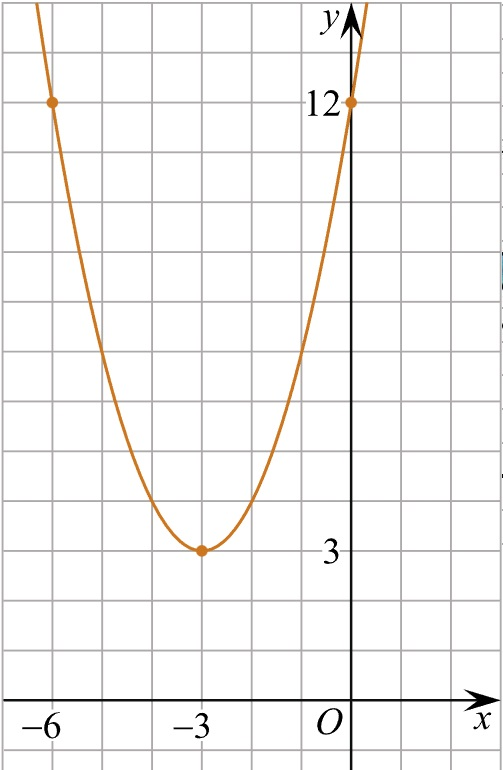
\includegraphics[align=t, width=\textwidth]{pics/G101M4C4-5.jpg}
		\end{minipage}
		\item
		\begin{minipage}[t]{0.66\textwidth}
			На рисунке изображён график функции вида \[ f(x)=\dfrac{a}{x+b}+c \], где числа \(a, b, c\) --- целые. Найдите \(f(10)\).
		\end{minipage}
		\hspace{0.05\textwidth}
		\begin{minipage}[t]{0.22\textwidth}
			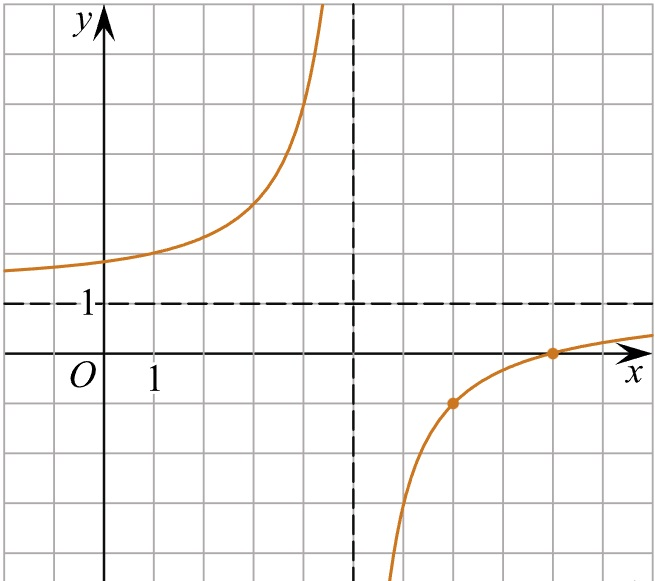
\includegraphics[align=t, width=\textwidth]{pics/G101M4H2-9.jpg}
		\end{minipage}
%		\item
%		\begin{minipage}[t]{0.66\textwidth}
%			На рисунке изображён график функции вида \[ f(x)=a+\dfrac{b}{x-c} \], где числа \(a, b, c\) --- целые. Найдите \(f(-6)\).
%		\end{minipage}
%		\hspace{0.05\textwidth}
%		\begin{minipage}[t]{0.22\textwidth}
%			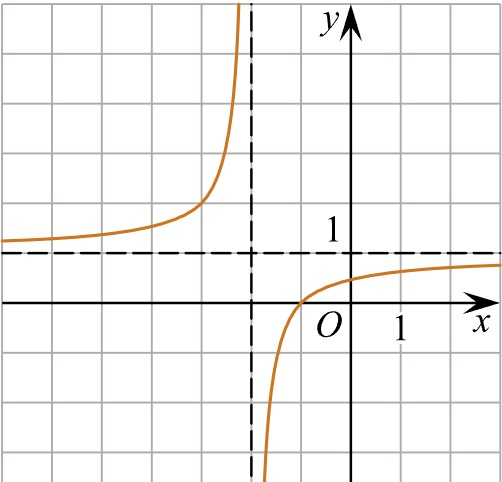
\includegraphics[align=t, width=\textwidth]{pics/G101M4H2-10.jpg}
%		\end{minipage}
		\item
		\begin{minipage}[t]{0.66\textwidth}
			На рисунке изображён график функции вида \[ f(x)=\dfrac{ax+b}{x+c} \], где числа \(a, b, c\) --- целые. Найдите \(a\).
		\end{minipage}
		\hspace{0.05\textwidth}
		\begin{minipage}[t]{0.22\textwidth}
			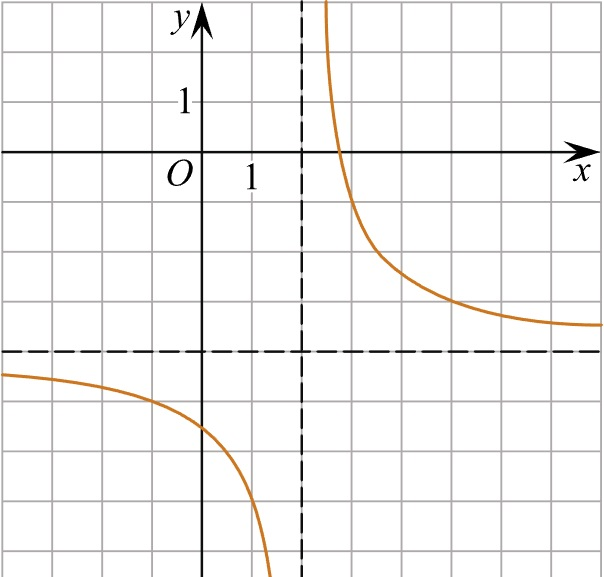
\includegraphics[align=t, width=\textwidth]{pics/G101M4H2-11.jpg}
		\end{minipage}
	\end{listofex}
\end{homework}

%===============>>  Занятие 3  <<===============
%
%\begin{class}[number=3]
%	\begin{listofex}
%		\item Пусто
%	\end{listofex}
%\end{class}
%
%===============>>  Занятие 4  <<===============
\begin{class}[number=4]
	\begin{listofex}
		\item
		\begin{minipage}[t]{0.67\textwidth}
			На рисунке изображён график функции \(f(x)=kx+b\). Найдите \(f(-9)\).
		\end{minipage}
		\begin{minipage}[c]{0.25\textwidth}
			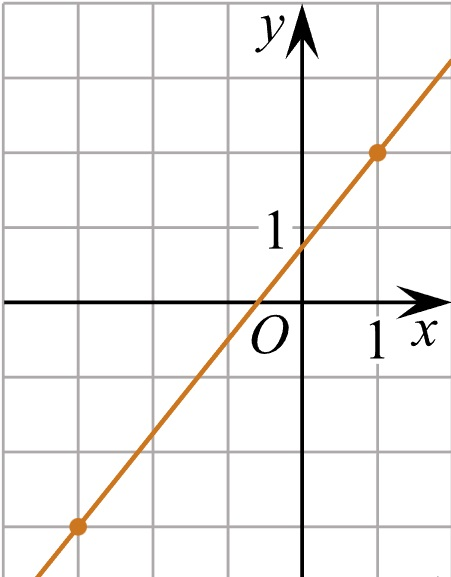
\includegraphics[align=t, width=\textwidth]{pics/G101M4C4-1.jpg}
		\end{minipage}
		\item
		\begin{minipage}[t]{0.82\textwidth}
			На рисунке изображены графики двух линейных функций. Найдите абсциссу точки пересечения графиков.
		\end{minipage}
		\begin{minipage}[c]{0.13\textwidth}
			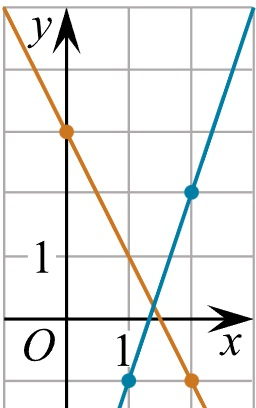
\includegraphics[align=t, width=\textwidth]{pics/G101M4C4-2.jpg}
		\end{minipage}
		\item
		\begin{minipage}[t]{0.67\textwidth}
			На рисунке изображён график функции вида \(f(x)=ax^2+bx+c\), где числа \(a, b, c\) --- целые. Найдите значение \(f(-3)\).
		\end{minipage}
		\begin{minipage}[c]{0.25\textwidth}
			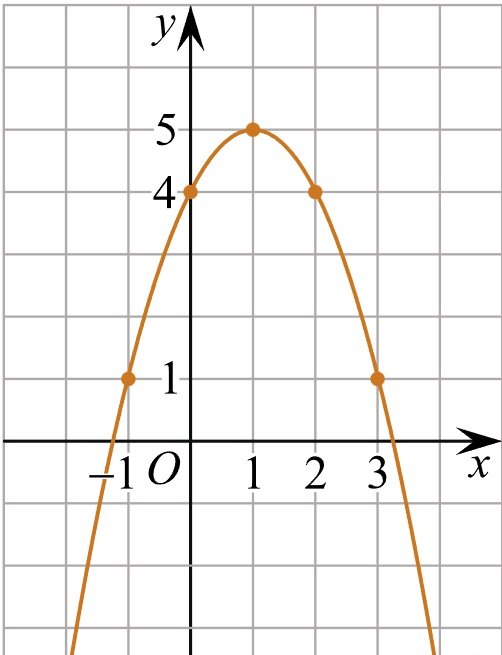
\includegraphics[align=t, width=\textwidth]{pics/G101M4C4-3.jpg}
		\end{minipage}
		\item
		\begin{minipage}[t]{0.67\textwidth}
			На рисунке изображён график функции вида \(f(x)=ax^2+bx+c\), где числа \(a, b, c\) --- целые. Найдите значение \(f(0,5)\).
		\end{minipage}
		\begin{minipage}[c]{0.25\textwidth}
			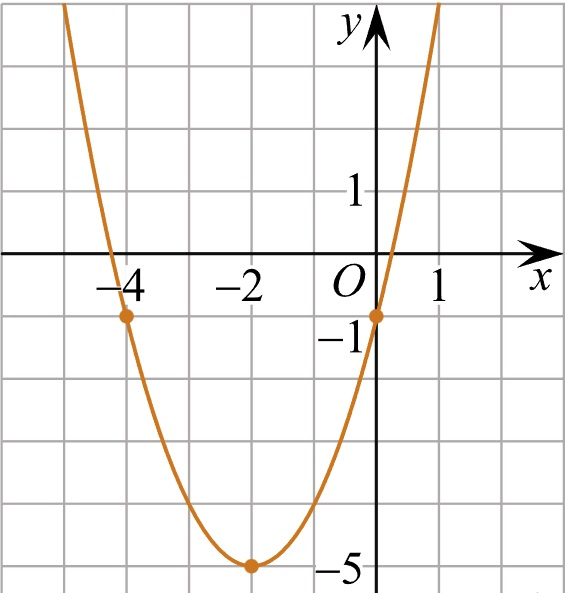
\includegraphics[align=t, width=\textwidth]{pics/G101M4C4-4.jpg}
		\end{minipage}
		\item
		\begin{minipage}[t]{0.67\textwidth}
			На рисунке изображён график функции вида \(f(x)=ax^2+bx+c\), где числа \(a, b, c\) --- целые. Найдите абсциссу вершины параболы.
		\end{minipage}
		\begin{minipage}[c]{0.25\textwidth}
			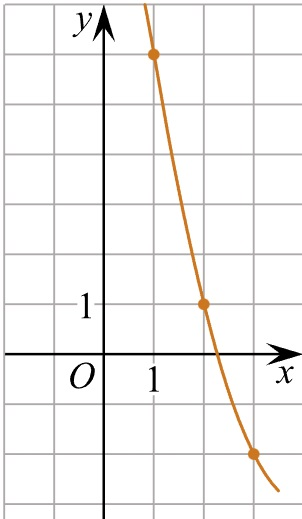
\includegraphics[align=t, width=\textwidth]{pics/G101M4C4-6.jpg}
		\end{minipage}
		\item
		\begin{minipage}[t]{0.67\textwidth}
			На рисунке изображён график функции вида \(f(x)=\dfrac{k}{x}+a\). Найдите \(f(-12)\).
		\end{minipage}
		\begin{minipage}[c]{0.25\textwidth}
			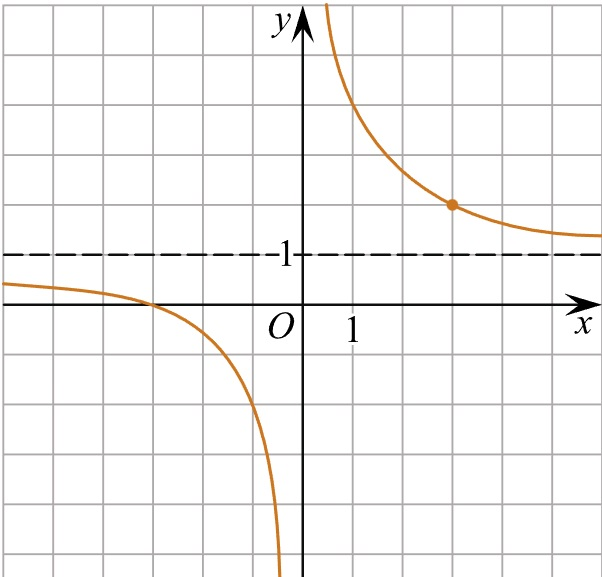
\includegraphics[align=t, width=\textwidth]{pics/G101M4C4-7.jpg}
		\end{minipage}
		\item
		\begin{minipage}[t]{0.67\textwidth}
			На рисунке изображён график функции вида \(f(x)=\dfrac{a}{x+b}+c\), где числа \(a, b, c\) --- целые. Найдите \(f(13)\).
		\end{minipage}
		\begin{minipage}[c]{0.25\textwidth}
			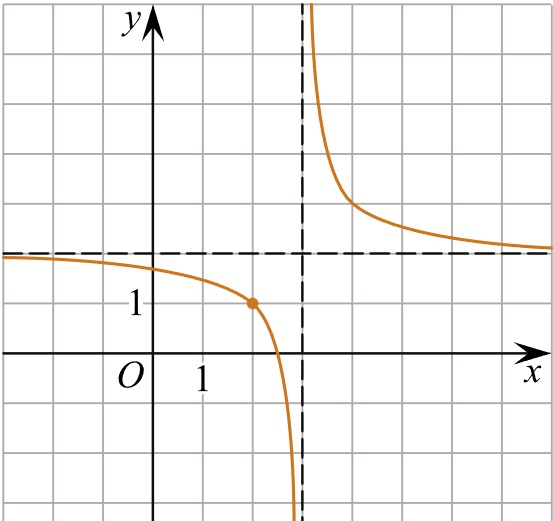
\includegraphics[align=t, width=\textwidth]{pics/G101M4C4-8.jpg}
		\end{minipage}
		\item
		\begin{minipage}[t]{0.67\textwidth}
			На рисунке изображён график функции вида \(f(x)=\dfrac{a}{x+b}+c\), где числа \(a, b, c\) --- целые. Найдите \(f(10)\).
		\end{minipage}
		\begin{minipage}[c]{0.25\textwidth}
			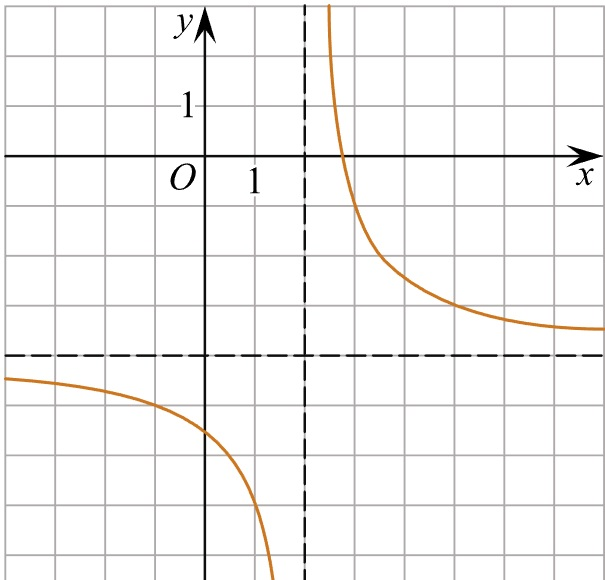
\includegraphics[align=t, width=\textwidth]{pics/G101M4C4-9.jpg}
		\end{minipage}
	\end{listofex}
\end{class}
%
%===============>>  Домашняя работа 2  <<===============
%
\begin{homework}[number=2]
	\begin{listofex}
		\item 
		\begin{minipage}[t]{0.67\textwidth}
			На рисунке изображён график функции \(f(x)=kx+b\). Найдите \(f(-5)\).
		\end{minipage}
		\begin{minipage}[c]{0.25\textwidth}
			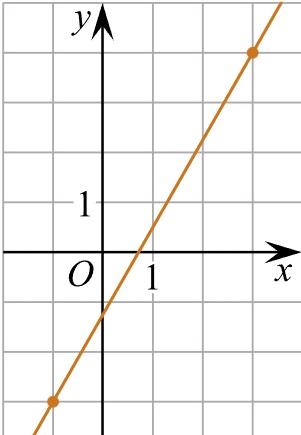
\includegraphics[width=\textwidth]{pics/G101M4H2-1.jpg}
		\end{minipage}
		\item 
		\begin{minipage}[t]{0.67\textwidth}
			На рисунке изображены графики двух линейных функций. Найдите абсциссу точки пересечения графиков.
		\end{minipage}
		\begin{minipage}[c]{0.25\textwidth}
			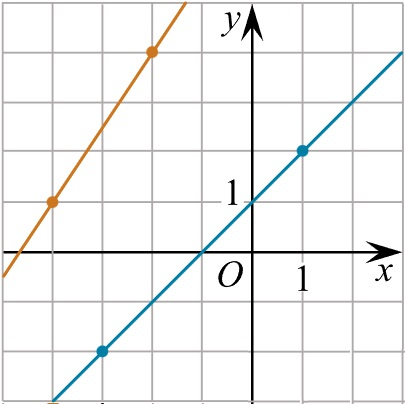
\includegraphics[width=\textwidth]{pics/G101M4H2-2.jpg}
		\end{minipage}
		\item 
		\begin{minipage}[t]{0.67\textwidth}
			На рисунке изображены графики двух линейных функций. Найдите абсциссу точки пересечения графиков.
		\end{minipage}
		\begin{minipage}[c]{0.25\textwidth}
			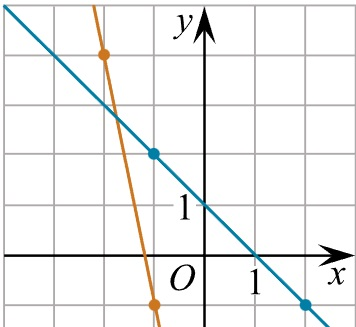
\includegraphics[width=\textwidth]{pics/G101M4H2-3.jpg}
		\end{minipage}
		\item
		\begin{minipage}[t]{0.67\textwidth}
			На рисунке изображён график функции вида \(f(x)=ax^2+bx+c\), где числа \(a, b, c\) --- целые. Найдите значение \(f(0,5)\).
		\end{minipage}
		\begin{minipage}[c]{0.25\textwidth}
			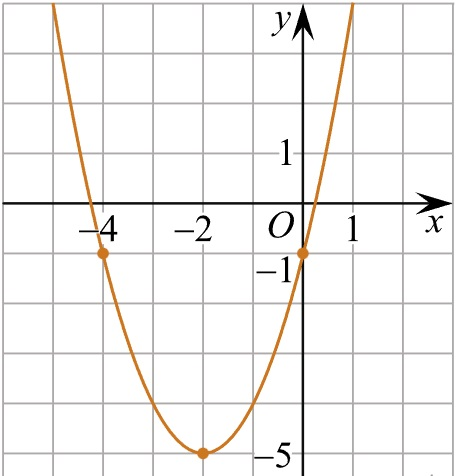
\includegraphics[width=\textwidth]{pics/G101M4H2-4.jpg}
		\end{minipage}
%		\item
%		\begin{minipage}[t]{0.67\textwidth}
%			На рисунке изображён график функции вида \(f(x)=ax+|bx+c|+d\), где числа \(a, b, c, d\) --- целые. Найдите корень уравнения \(bx+c=0\).
%		\end{minipage}
%		\begin{minipage}[c]{0.25\textwidth}
%			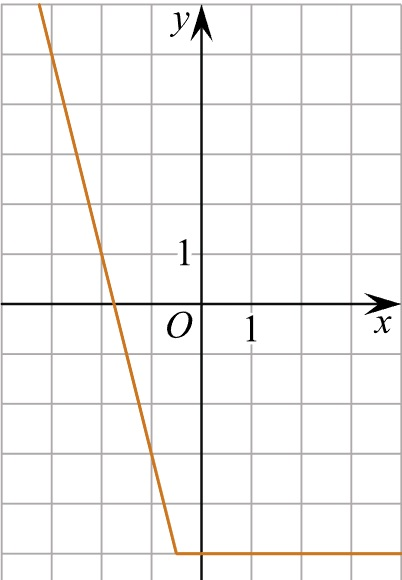
\includegraphics[width=\textwidth]{pics/G101M4H2-6.jpg}
%		\end{minipage}
%		\item
%		\begin{minipage}[t]{0.67\textwidth}
%			На рисунке изображён график функции вида \(f(x)=ax-|bx+c|+d\), где числа \(a, b, c, d\) --- целые. Найдите корень уравнения \(ax=d\).
%		\end{minipage}
%		\begin{minipage}[c]{0.25\textwidth}
%			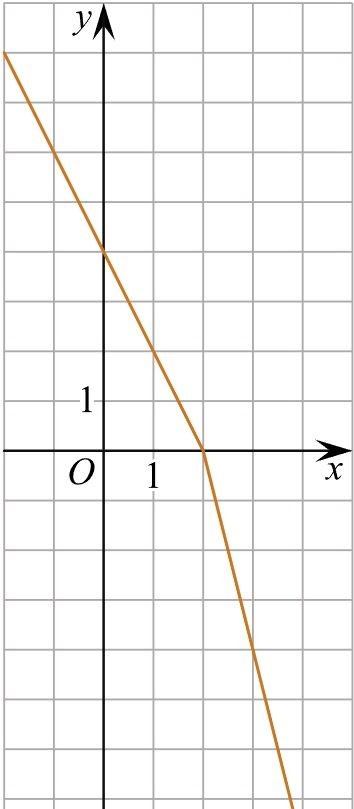
\includegraphics[width=\textwidth]{pics/G101M4H2-7.jpg}
%		\end{minipage}
%		\item
%		\begin{minipage}[t]{0.67\textwidth}
%			На рисунке изображён график функции вида \(f(x)=ax-|bx+c|+d\), где числа \(a, b, c, d\) --- целые. Найдите корень уравнения \(ax+d=0\).
%		\end{minipage}
%		\begin{minipage}[c]{0.25\textwidth}
%			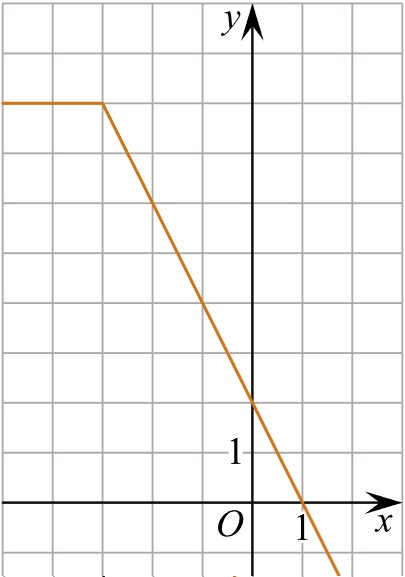
\includegraphics[width=\textwidth]{pics/G101M4H2-8.jpg}
%		\end{minipage}
	\end{listofex}
\end{homework}
%
%===============>>  Занятие 5  <<===============
\begin{class}[number=5]
	\begin{listofex}
		\item
		\begin{minipage}[t]{0.66\textwidth}
			На рисунке изображён график функции вида \[ f(x)=\dfrac{k}{x}+a \]. Найдите, при каком значение \(x)\) значение функции равно \(0,8\).
		\end{minipage}
		\hspace{0.05\textwidth}
		\begin{minipage}[t]{0.22\textwidth}
			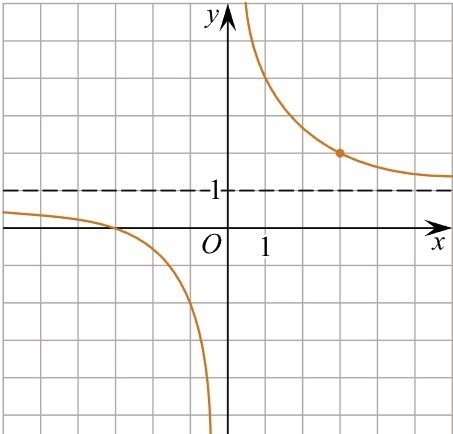
\includegraphics[align=t, width=\textwidth]{pics/G101M4C5-1.jpg}
		\end{minipage}
		\item
		\begin{minipage}[t]{0.66\textwidth}
			На рисунке изображён график функции вида \[ f(x)=\dfrac{k}{x+b}+a \], где числа \(a, b, c\) --- целые. Найдите \(f(9)\).
		\end{minipage}
		\hspace{0.05\textwidth}
		\begin{minipage}[t]{0.22\textwidth}
			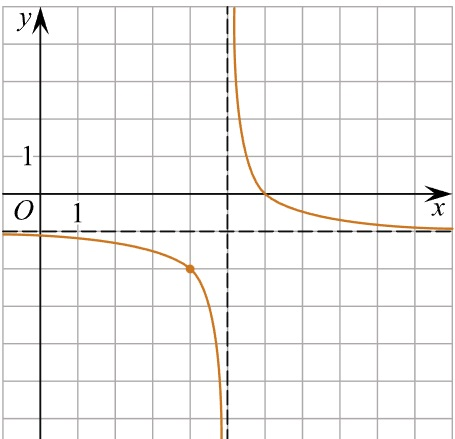
\includegraphics[align=t, width=\textwidth]{pics/G101M4C5-2.jpg}
		\end{minipage}
		\item
		\begin{minipage}[t]{0.66\textwidth}
			На рисунке изображён график функции вида \[ f(x)=\dfrac{k}{x+b}+a \], где числа \(a, b, c\) --- целые. Найдите \(f(4)\).
		\end{minipage}
		\hspace{0.05\textwidth}
		\begin{minipage}[t]{0.22\textwidth}
			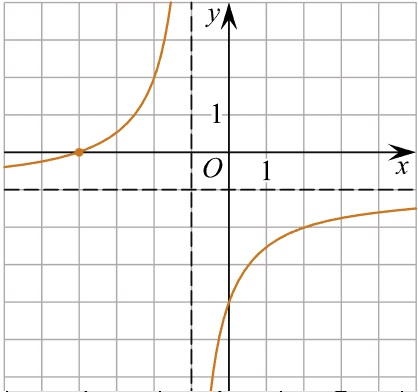
\includegraphics[align=t, width=\textwidth]{pics/G101M4C5-3.jpg}
		\end{minipage}
		\item
		\begin{minipage}[t]{0.66\textwidth}
			На рисунке изображён график функции вида \[ f(x)=\dfrac{ax+b}{x+c} \], где числа \(a, b, c\) --- целые. Найдите \(a\).
		\end{minipage}
		\hspace{0.05\textwidth}
		\begin{minipage}[t]{0.22\textwidth}
			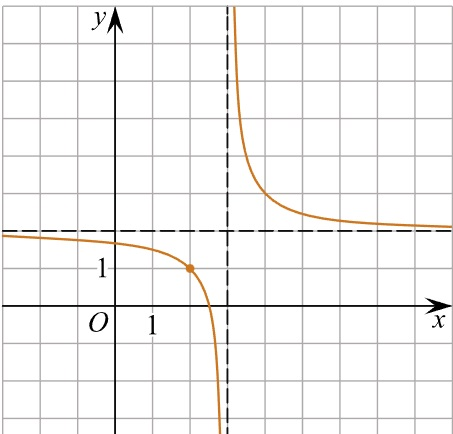
\includegraphics[align=t, width=\textwidth]{pics/G101M4C5-4.jpg}
		\end{minipage}
		\item
		\begin{minipage}[t]{0.66\textwidth}
			На рисунке изображён график функции вида \[ f(x)=\dfrac{ax+b}{x+c} \], где числа \(a, b, c\) --- целые. Найдите \(a\).
		\end{minipage}
		\hspace{0.05\textwidth}
		\begin{minipage}[t]{0.22\textwidth}
			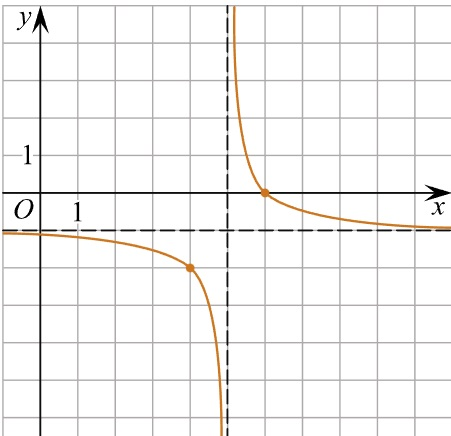
\includegraphics[align=t, width=\textwidth]{pics/G101M4C5-5.jpg}
		\end{minipage}
		\item
		\begin{minipage}[t]{0.66\textwidth}
			На рисунке изображён график функции вида \(f(x)=ax^2+bx+c\), где числа \(a, b, c\) --- целые. Найдите значение \(f(6,5)\).
		\end{minipage}
		\hspace{0.05\textwidth}
		\begin{minipage}[t]{0.22\textwidth}
			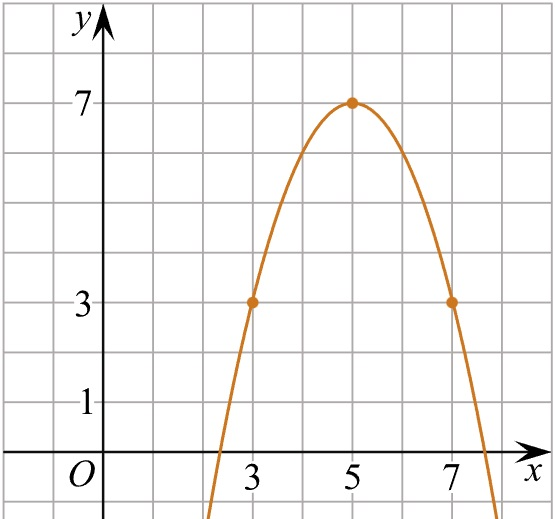
\includegraphics[width=\textwidth]{pics/G101M4H2-5.jpg}
		\end{minipage}
		\item Высота над землeй подброшенного вверх мяча меняется по закону \(h(t)=1,6+8t-5t^2\) где \(h\) --- высота в метрах, \(t\) --- время в секундах, прошедшее с момента броска. Сколько секунд мяч будет
		находиться на высоте не менее трeх метров?
		\item \exercise{1540}
%		\item
%		\begin{minipage}[t]{0.66\textwidth}
%			На рисунке изображён график функции вида \[ f(x)=ax+|bx+c|+d \], где числа \(a, b, c, d\) --- целые. Найдите корень уравнения \(ax+d=0\).
%		\end{minipage}
%		\hspace{0.05\textwidth}
%		\begin{minipage}[t]{0.22\textwidth}
%			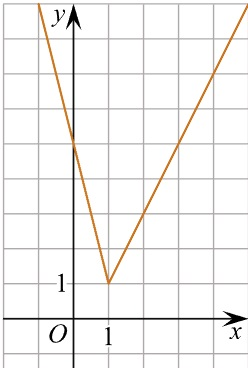
\includegraphics[align=t, width=\textwidth]{pics/G101M4C5-6.jpg}
%		\end{minipage}
%		\item
%		\begin{minipage}[t]{0.66\textwidth}
%			На рисунке изображён график функции вида \[ f(x)=ax+|bx+c|+d \], где числа \(a, b, c, d\) --- целые. Найдите корень уравнения \(ax+d=0\).
%		\end{minipage}
%		\hspace{0.05\textwidth}
%		\begin{minipage}[t]{0.22\textwidth}
%			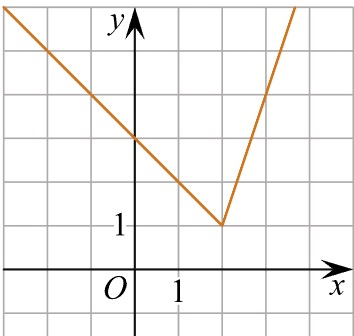
\includegraphics[align=t, width=\textwidth]{pics/G101M4C5-7.jpg}
%		\end{minipage}
%		\item
%		\begin{minipage}[t]{0.66\textwidth}
%			На рисунке изображён график функции вида \[ f(x)=ax+|bx+c|+d \], где числа \(a, b, c, d\) --- целые. Найдите корень уравнения \(ax+d=0\).
%		\end{minipage}
%		\hspace{0.05\textwidth}
%		\begin{minipage}[t]{0.22\textwidth}
%			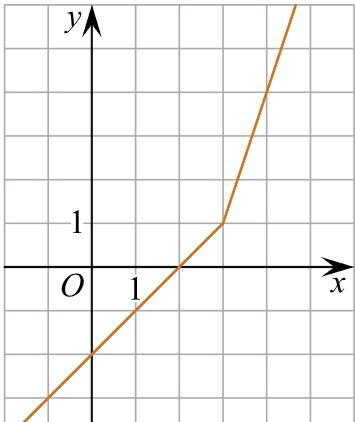
\includegraphics[align=t, width=\textwidth]{pics/G101M4C5-8.jpg}
%		\end{minipage}
%		\item
%		\begin{minipage}[t]{0.66\textwidth}
%			На рисунке изображён график функции вида \[ f(x)=ax+|bx+c|+d \], где числа \(a, b, c, d\) --- целые. Найдите корень уравнения \(ax+d=19\).
%		\end{minipage}
%		\hspace{0.05\textwidth}
%		\begin{minipage}[t]{0.22\textwidth}
%			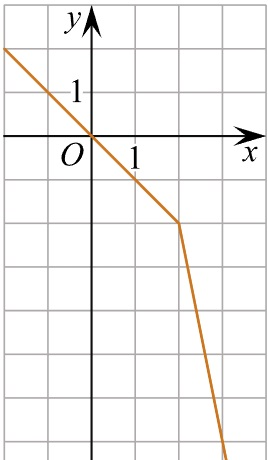
\includegraphics[align=t, width=\textwidth]{pics/G101M4C5-9.jpg}
%		\end{minipage}
%		\item
%		\begin{minipage}[t]{0.66\textwidth}
%			На рисунке изображён график функции вида \[ f(x)=ax+|bx+c|+d \], где числа \(a, b, c, d\) --- целые. Найдите корень уравнения \(ax=d\).
%		\end{minipage}
%		\hspace{0.05\textwidth}
%		\begin{minipage}[t]{0.22\textwidth}
%			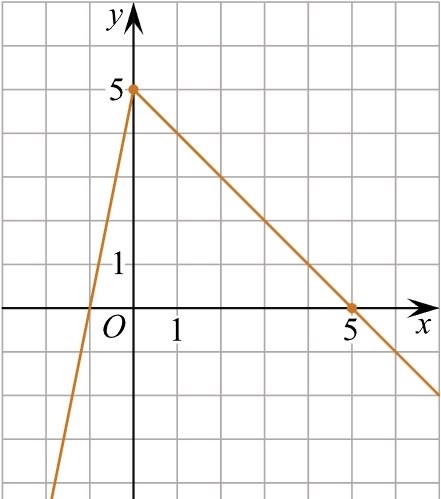
\includegraphics[align=t, width=\textwidth]{pics/G101M4C5-10.jpg}
%		\end{minipage}
	\end{listofex}
\end{class}
%
%===============>>  Домашняя работа 3  <<===============
%
%\begin{homework}[number=2]
%	\begin{listofex}
%
%	\end{listofex}
%\end{homework}
%\newpage
%\title{Подготовка к проверочной работе}
%\begin{listofex}
%	
%\end{listofex}
%
%===============>>  Занятие 6  <<===============
%
\begin{class}[number=6]
	\begin{listofex}
		\item Решить систему неравенств:
		\[ \left\{
		\begin{array}{l}
			5(4x+3)-3(4x+5)\le8x+9,\\
			\dfrac{x+2}{4}+\dfrac{x+4}{2}\ge\dfrac{x+3}{5}+\dfrac{x+5}{3}.
		\end{array}
		\right. \]
		\item Решите двойное неравенство: \( 2x+3\le5x^2-9x+5\le7x+2 \).
		\item
		\begin{minipage}[t]{\bodywidth}
			На рисунке изображён график функции \(f(x)=kx+b\). Найдите \(f(-9)\).
		\end{minipage}
		\hspace{0.02\linewidth}
		\begin{minipage}[t]{\picwidth}
			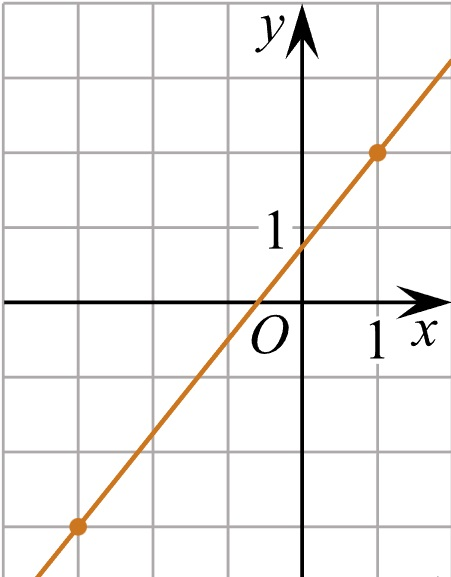
\includegraphics[align=t, width=\textwidth]{pics/G101M4C4-1.jpg}
		\end{minipage}
%		В ДЗ
%		\item
%		\begin{minipage}[t]{\bodywidth}
%			На рисунке изображён график функции вида \[ f(x)=ax+|bx+c|+d, \] где числа \(a, b, c, d\) --- целые. Найдите корень уравнения \(ax+d=10\).
%		\end{minipage}
%		\hspace{0.02\linewidth}
%		\begin{minipage}[t]{\picwidth}
%			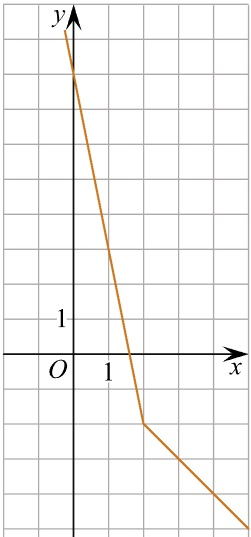
\includegraphics[align=t, width=\linewidth]{pics/G101M4C6-1.jpg}
%		\end{minipage}
		\item
		\begin{minipage}[t]{\bodywidth}
			На рисунке изображён график функции вида \(f(x)=ax^2+bx+c\), где числа \(a, b, c\) --- целые. Найдите значение \(f\left( -\mfrac{1}{1}{2} \right)\).
		\end{minipage}
		\hspace{0.02\linewidth}
		\begin{minipage}[t]{\picwidth}
			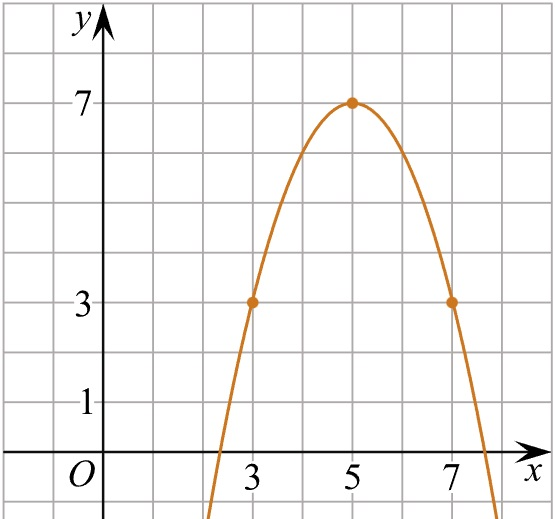
\includegraphics[align=t, width=\linewidth]{pics/G101M4H2-5.jpg}
		\end{minipage}
		\item
		\begin{minipage}[t]{\bodywidth}
			На рисунке изображён график функции вида \[ f(x)=ax+|bx+c|+d, \] где числа \(a, b, c, d\) --- целые. Найдите корень уравнения \(ax+d=-15\).
		\end{minipage}
		\hspace{0.02\linewidth}
		\begin{minipage}[t]{\picwidth}
			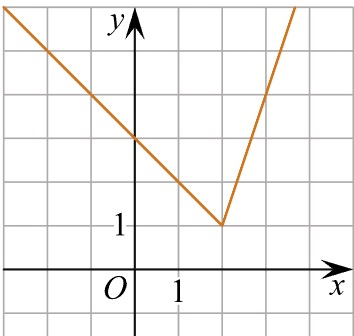
\includegraphics[align=t, width=\linewidth]{pics/G101M4C5-7.jpg}
		\end{minipage}
		\item
		\begin{minipage}[t]{\bodywidth}
			На рисунке изображён график функции вида \[ f(x)=ax+|bx+c|+d, \] где числа \(a, b, c, d\) --- целые. Найдите корень уравнения \(bx+c=2\).
		\end{minipage}
		\hspace{0.02\linewidth}
		\begin{minipage}[t]{\picwidth}
			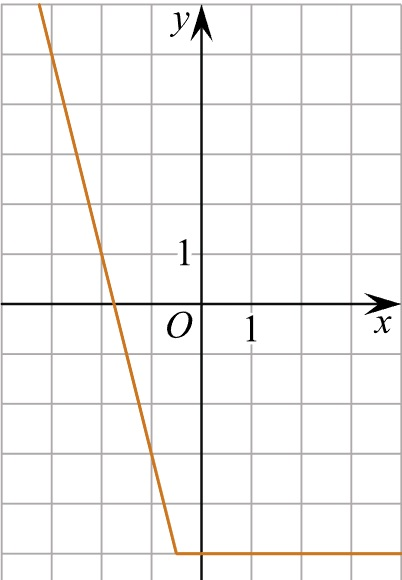
\includegraphics[align=t, width=\linewidth]{pics/G101M4H2-6.jpg}
		\end{minipage}
		\item
		\begin{minipage}[t]{\bodywidth}
			На рисунке изображён график функции вида \[ f(x)=ax-|bx+c|+d, \] где числа \(a, b, c, d\) --- целые. Найдите корень уравнения \(ax+d=-2\).
		\end{minipage}
		\hspace{0.02\linewidth}
		\begin{minipage}[t]{\picwidth}
			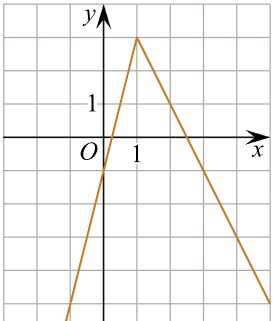
\includegraphics[align=t, width=\linewidth]{pics/G101M4C6-8.jpg}
		\end{minipage}
		\item
		\begin{minipage}[t]{\bodywidth}
			На рисунке изображён график функции вида \[ f(x)=\dfrac{a}{x+b}+c, \] где числа \(a, b, c\) --- целые. Найдите значение \(x\), при котором \(f(x)=-5\).
		\end{minipage}
		\hspace{0.02\linewidth}
		\begin{minipage}[t]{\picwidth}
			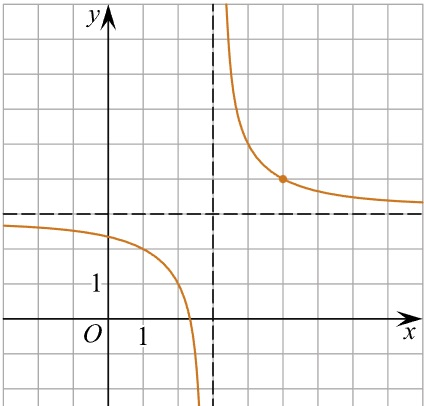
\includegraphics[align=t, width=\linewidth]{pics/G101M4C6-2.jpg}
		\end{minipage}
%		В ДЗ
%		\item
%		\begin{minipage}[t]{\bodywidth}
%			На рисунке изображён график функции вида \[ f(x)=\dfrac{a}{x+b}+c, \] где числа \(a, b, c\) --- целые. Найдите значение \(x\), при котором \(f(x)=2,5\).
%		\end{minipage}
%		\hspace{0.02\linewidth}
%		\begin{minipage}[t]{\picwidth}
%			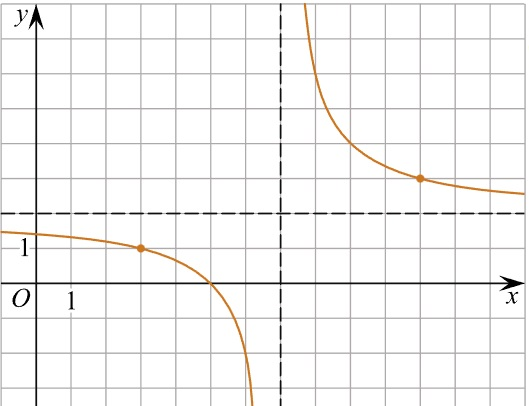
\includegraphics[align=t, width=\linewidth]{pics/G101M4C6-3.jpg}
%		\end{minipage}
%		\item
%		\begin{minipage}[t]{\bodywidth}
%			На рисунке изображён график функции вида \[ f(x)=\dfrac{a}{x+b}+c, \] где числа \(a, b, c\) --- целые. Найдите значение \(x\), при котором \(f(x)=-1,125\).
%		\end{minipage}
%		\hspace{0.02\linewidth}
%		\begin{minipage}[t]{\picwidth}
%			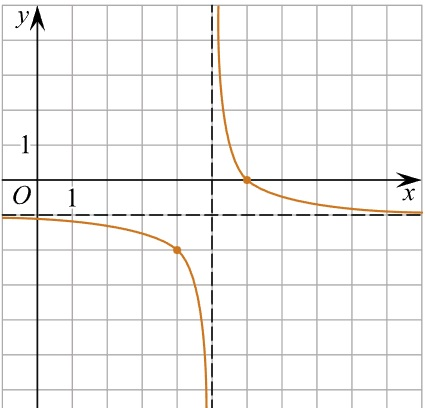
\includegraphics[align=t, width=\linewidth]{pics/G101M4C6-4.jpg}
%		\end{minipage}
		\item
		\begin{minipage}[t]{\bodywidth}
			На рисунке изображён график функции вида \[ f(x)=\dfrac{ax+b}{x+c}, \] где числа \(a, b, c\) --- целые. Найдите \(b\).
		\end{minipage}
		\hspace{0.02\linewidth}
		\begin{minipage}[t]{\picwidth}
			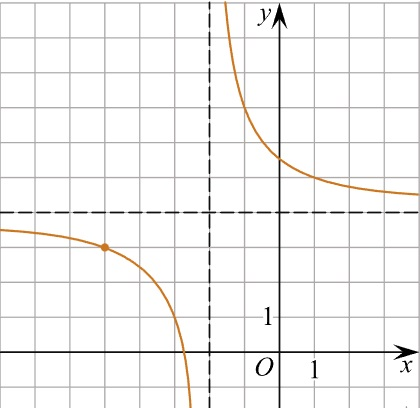
\includegraphics[align=t, width=\linewidth]{pics/G101M4C6-5.jpg}
		\end{minipage}
%		\item
%		\begin{minipage}[t]{\bodywidth}
%			На рисунке изображён график функции вида \[ f(x)=\dfrac{ax+b}{x+c}, \] где числа \(a, b, c\) --- целые. Найдите \(b\).
%		\end{minipage}
%		\hspace{0.02\linewidth}
%		\begin{minipage}[t]{\picwidth}
%			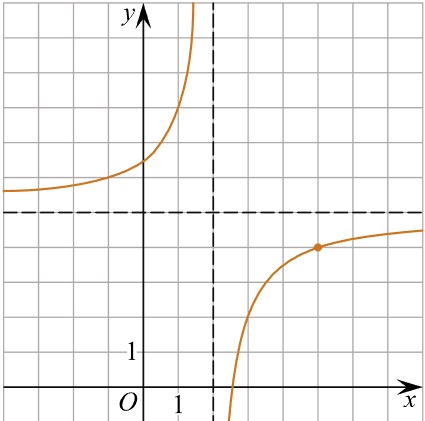
\includegraphics[align=t, width=\linewidth]{pics/G101M4C6-6.jpg}
%		\end{minipage}
%		\item
%		\begin{minipage}[t]{\bodywidth}
%			На рисунке изображён график функции вида \[ f(x)=\dfrac{ax+b}{x+c}, \] где числа \(a, b, c\) --- целые. Найдите \(b\).
%		\end{minipage}
%		\hspace{0.02\linewidth}
%		\begin{minipage}[t]{\picwidth}
%			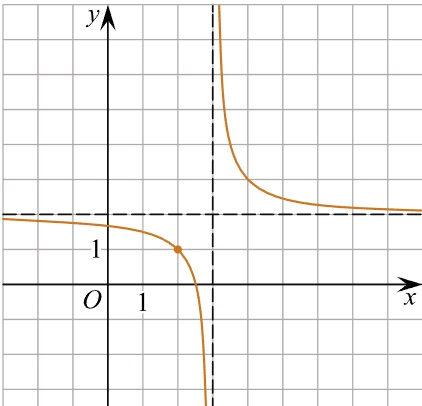
\includegraphics[align=t, width=\linewidth]{pics/G101M4C6-7.jpg}
%		\end{minipage}
	\end{listofex}
\end{class}
%
%===============>>  Провечная работа  <<===============
%
%\begin{exam}
%	\begin{listofex}
%	
%	\end{listofex}
%\end{exam}